\chapter{Introduction}

\section{Motivation}
% Search is amazing, ability to reason given limitied information, we can do many things without
% fully observing our environment. 
% Examples where partial observability is everywhere in the world and how we as humans have to deal 
% with it on a day to day basis which almost second nature to use. We do not have to think about it, we 
% just do it. This is increadibly difficult to do for robots, acting and reasing given incomplete information
% is one of the most challanging aspects of artificel intiellegence. Because of the sheer branching factor. 
% 
% Neuroscience evidence 
%
% Long-term and short term memory
%
%
% When reasoning with respect to uncertainty, number of assumptions are made
%

%
% 1) Describe uncertainty & risk in the world how important it is for biological entities to approprietly take it 
%    into account for survivial.  
%
%    Description of what humans are able to do on a day to day basis and how important uncertainty is Balancing risk.
%    Evidence of humans being expectation maximisers.
%
% 2) 
%

% An action is the result of two hidden states; Our beliefs and desires.

%
% 3) How is uncertainty handles in artificel intelligence ?
%
%
%
% 4) Uncertainty in robotics; how is it handled.
%
%
% 5) Summary

% 1)
Taking long term decisions or spontaneous reactive actions when presented with incomplete information or partial knowledge is 
paramount to the survival of any biological entity. Reasoning given uncertainty is a continuously occurring event throughout our 
livelihood. When considering long term decisions an abundance of examples come to mind; In economic investments 
uncertainty is, to the best of efforts, quantified and minimised. Reactive actions are just as common; When looking for the snooze button of an 
alarm clock, early in the morning, our hand seems to autonomously search the surrounding space, picking up sensory cues, gradually acquiring information 
which we utilise (or not) to guide us towards the button; Trying to connect a plug to a an occluded power socket under a desk, whilst 
being crouched, requires the integration of perceptions into a belief such to quantify the uncertainty which we can act upon to 
achieve the connection. Abilities close to these are not yet present in Artificial intelligence (AI) \& robotics.
% Need to say that we would fucking whish that robots are just as good as humans.
% 2) Neuroscience (how is the uncertainty and decision process modelled so fare)


It is not yet fully understood how decisions are taken; yet alone under uncertainty. The difficulty is that two processes responsible 
for the synthesis of our actions, our beliefs and desires, are not directly measurable. The first attempt at modelling the humans 
decision making process was in mathematics \& economics (\cite{Bernoulli1954},\cite{VonNeumann1944}), where emphasis was on 
predicting discrete choices formulated as a gamble. It is only recently in Motion and Neuroscience that more incites have 
been gained.

% . In locomotion behaviour uncertainty plays a role on how we plan our paths, there is evidence 
%in Neuroscience that the hypocampus plays an important role our internal representation.


% Understanding and subsequently predicting the way we reason 
% with respect to uncertainty and de facto how we handle risk has been modelled by a utility function and the probabilistic outcome 
% of our decisionse

% Should speak about evidence of neuroscience activity during locomotion. Do we know which parts of the brain are being 
% triggered when we are doing search. Is there neuroscience evidence of an internal map representation in our brain 
% ego-centric allocentric represenation (
 
% 3) Aritficiel intelligence & robots (How is uncertainty taken into account in the decision process)
Artificial intelligence \& robotics considered early on uncertainty in decision making, 
where the predominant application domain was spatial navigation (\cite{ActingUncertainty_1996}). The problem is composed 
into of two parts: the construction and representation of a world model (the map) and a planner which can reason with 
respect to this model such to accomplish an objective. The world construction problem  has attracted a large amount of 
research with many successfully applications in a wide spectrum of robotic domains (AUV,UAV,etc..). The planning problem 
is less well developed and is based on either representing the decision problem as a partially observable markov decision 
process (POMDP) which are notoriously difficult to solve for large scale problems, or through search heuristics.  
The mapping problem can generally be solved when assuming the uncertainty is Gaussian and thus quantifiable 
by a few parameters and the uncertainty originates from the imprecision of the sensors. As for the planning problem solutions are feasible
under the restrictive assumption of a discretization of the world, observations and actions of the robot. As a result there are very
few examples where uncertainty is considered in an optimal decision make process when considering a continuous state, action 
and observation space.

In summary there are still open problems in decision making when considering partial observability, whilst 
the mapping problem has been studied under a constraining set of assumptions. In this thesis we address both problems 
under extreme levels of uncertainty. 
For the decision making side we leverage humans foresight and reasoning in a Learning from Demonstration (LfD) (\cite{Billard08chapter})
framework, which is used to transfer skills from an expert teacher (usually a human) to a robot. Examples include the transfer of 
kinematic task constraints, stiffness and impedance constraints and motion primitives, just to name a few.
It has been shown, for the moment being, both humans and animals are far better at navigation than robots especially when 
uncertainty is present (\cite{stankiewicz2006lost}). For the mapping problem we develop a Bayesian filter which is non-parametric 
and has no explicit representation of a joint distribution.

\begin{figure}
 \centering
 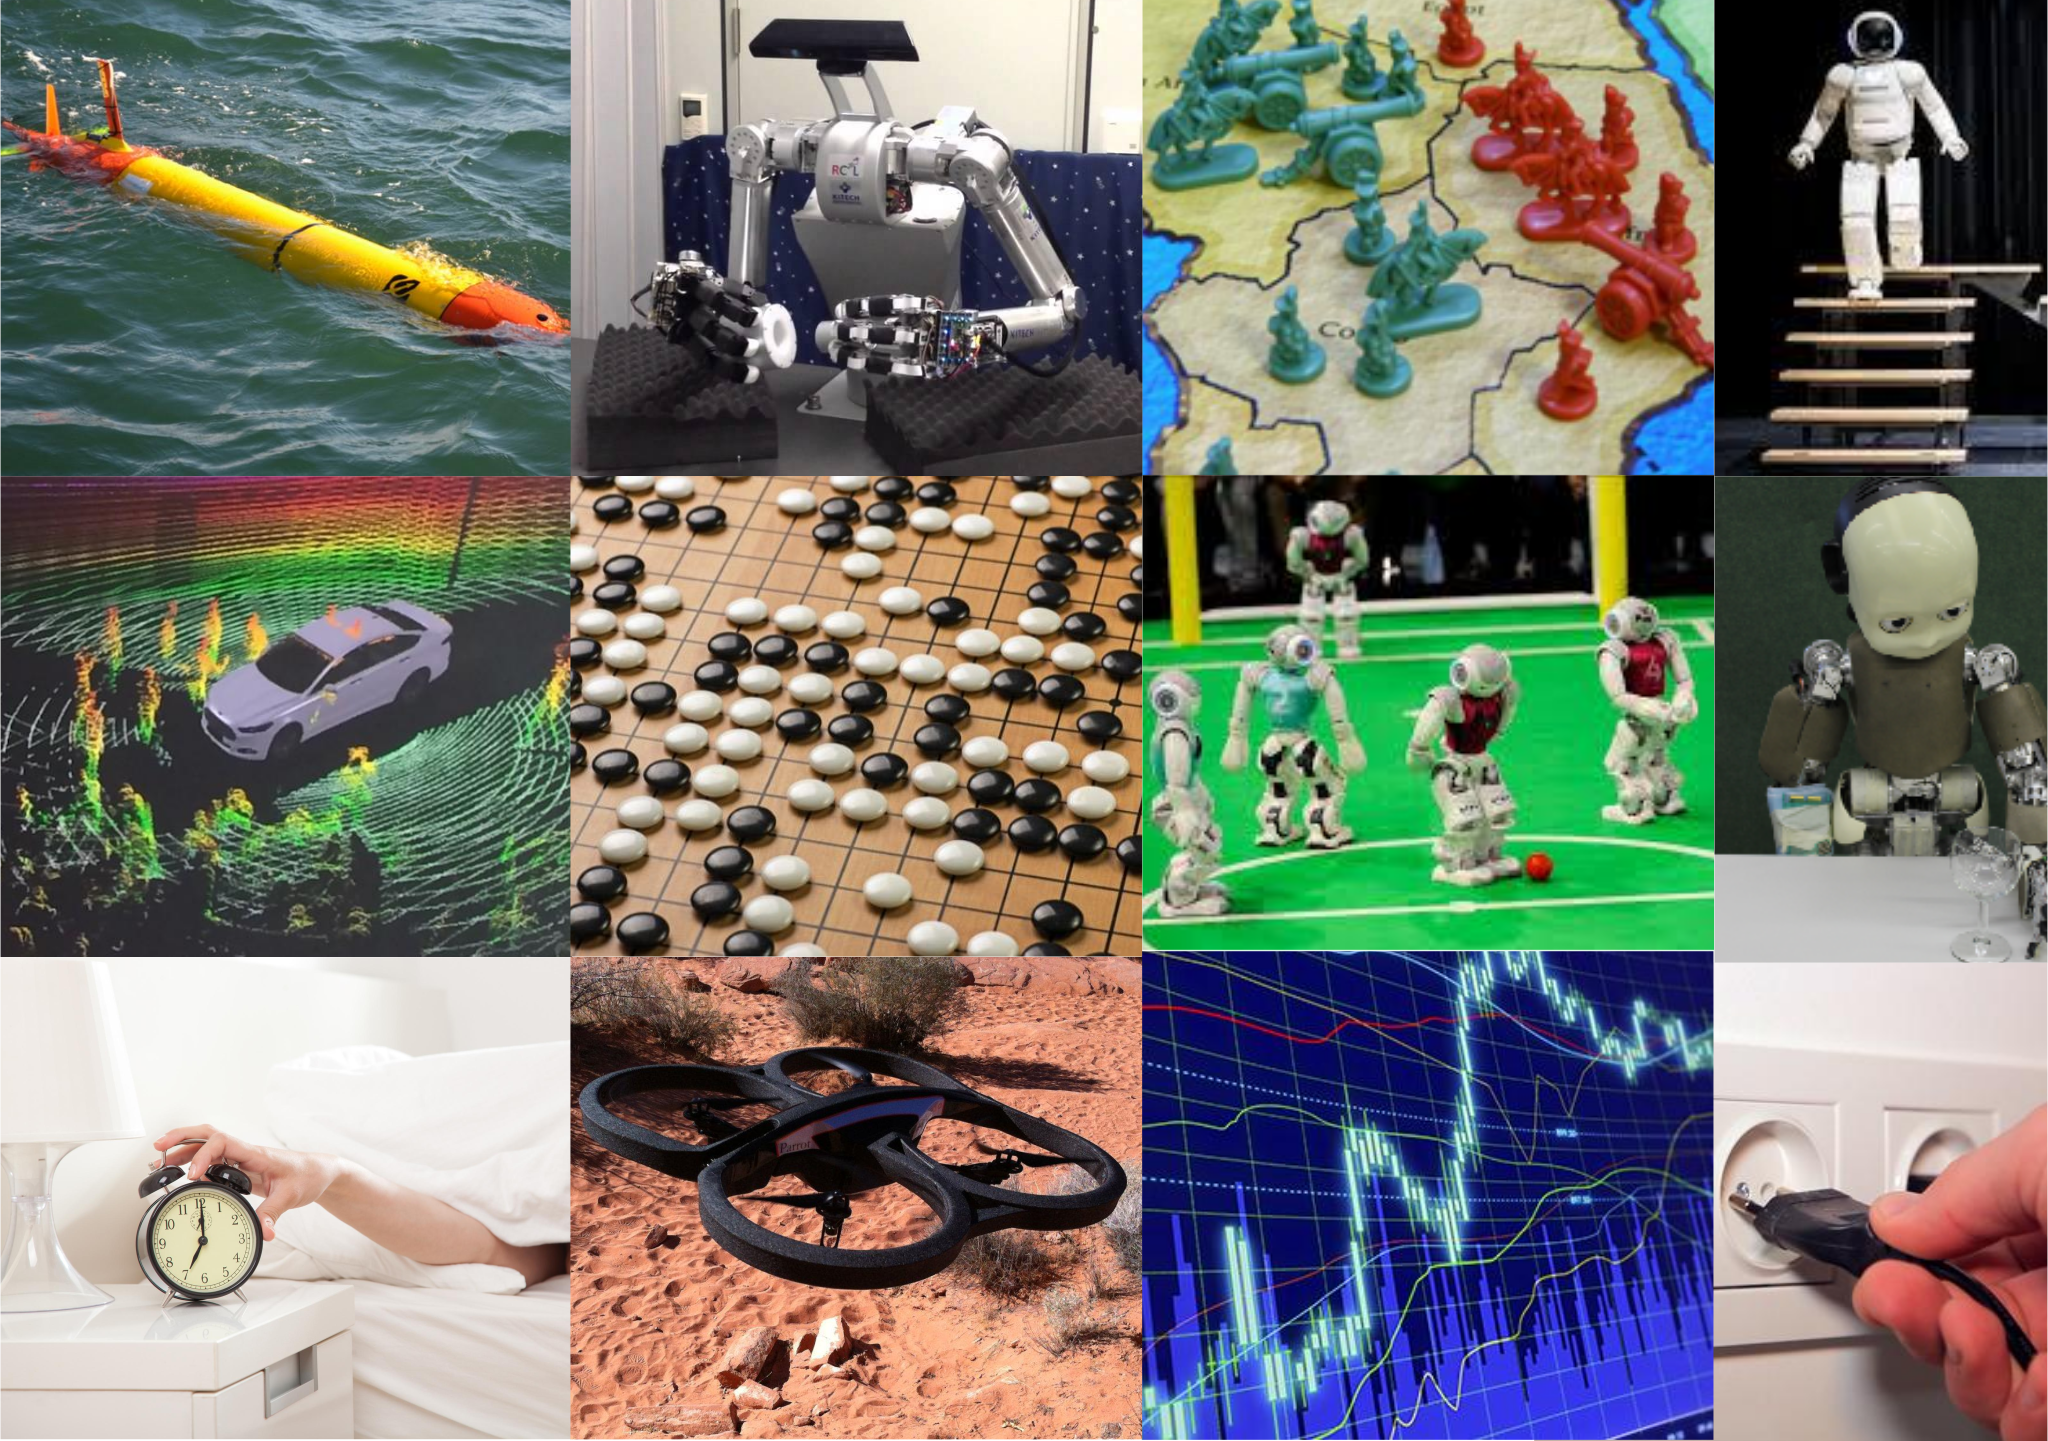
\includegraphics[width=0.8\textwidth]{examples.pdf}
\end{figure}


%The advantage of taking a LfD approach and encoding the demonstrated behaviour in a asynchronous dynamical system (ADS) is that we have robustness to perturbation
% and a generalisation over the entire state space. 

\section{Contribution}
% - One page 1/2 

In this thesis we bring to light two main ideas. The first is the transfer of human behaviour to robots
in tasks where a lot of uncertainty in present, making them difficult to solve using traditional techniques.
The second is a non-parametric Bayesian state space filter.

Throughout the work in this thesis we consider case studies in which vision is not available; leaving tactile and 
haptic information. This choice was made to induce a high level of uncertainty making it easier to study. As 
a consequence the tasks we consider are by nature, haptic and tactile searches.

\subsection{Learning to reason with uncertainty as humans}

A Markov Decision Process (MDP) allows to formulate a decision problem in terms of states, actions, a discount factor 
and a cost function. Given this formulation and a suitable optimisation method (dynamic programming, temporal difference, etc..) 
a set of optimal decision rules are returned, known as a policy. The benefit of this approach 
is that the policy is non-myopic and realises the importance of initial sub-optimal actions which might at first 
be necessary to achieve the task in the long run. A Partially Observable Markov Decision Process (POMDP), is 
a generalisation of an MDP to a hidden state space and only observation are available relating 
to the state space. An exact solution to a POMDP is only feasible in simple toy problems 
(\cite{Thrun_Burgard_Fox_2005}) and existing approximate solutions are tailored for discretized 
representation of states, actions and observations.

In this thesis we propose a Learning from Demonstration approach to solving the POMDP problem in
haptic and tactile search tasks. Our hypothesis is that if we know the mental state of the human 
expert in terms of his believed location and observe his actions we can learn a statistical policy 
which mimics his behaviour. Since the human's beliefs are not directly observable we infer them 
by assuming that the way we integrate behaviour is similar to a Bayesian filter. There is   
evidence both in cognitive and neuroscience that this is the case (\cite{Bake_Saxe_Tene_2011}). From 
the expert human demonstrations of the task we learn a cognitive model of the humans decision process 
by learning a generative joint distribution over his beliefs and actions. The generative distribution 
is then used as a control policy. By this approach we are able to have a policy which can handle uncertainty
similarly to humans. 

\subsection{Non-parametric Bayesian state space filter}

Simultaneous Localisation and Mapping (SLAM) is concerned with the development of filters to accurately and efficiently infer 
the state parameters (position, orientation,...) of an agent and aspects of its environment, commonly referred to as the map. 
It is necessary for the agent to achieve situatedness which is a precondition to planning and reasoning. The 
predominant usage of SLAM algorithm make the assumption that uncertainty is related to the noise in the sensor measurements. In 
our haptic search tasks there is no visual information and a very large amount of uncertainty. Most of the sensory
feedback is negative information, a term used to denote the non event of a sensor response from the objects (aka landmarks) in question.
In the absence of recurrent sightings or direct measurements of objects there are no correlations from the measurement errors 
which can be exploited. 

In this thesis we propose a new SLAM filter, which we name Measurement Likelihood Memory Filter (MLMF), in 
which no assumptions are taken with respect to the shape of the uncertainty (it can be Gaussian, multi-modal, uniform, etc..) and 
motion noise. From the loose assumptions we stipulate regarding the marginals, we adopt a histogram parametrisation (this is considered non-parametric 
because a change in a parameter has a local effect). The conceptual difference between the MLMF and standard SLAM filters 
such as EKF is that we avoid representing the joint distribution since it would entail a shattering space and time complexity. 
This is achieved by keeping track of the history of measurement likelihood functions. We demonstrate that our approach gives 
the same filtered marginals as a histogram filter. In such a way we achieve a Bayes filter which has both linear space and 
time complexity. This filter is well suited to tasks where the landmarks are not directly observable.

\subsection{Reinforcement learning in belief space}

We propose a Reinforcement Learning framework for the task of searching and connection a power plug to a socket, with only haptic 
and tactile information. We previously addressed this setup by learning a generative model of the beliefs and actions with data 
provide by human demonstrations following the LfD approach. However, it is usually the requirement in such setups that 
the teach is an expert, with few notable exceptions (\cite{rai2013learning}). Since we were solely learning a 
statistical controller, bad and good demonstrations will be mixed in together. By introducing a cost function 
representing the task we can explicitly have a quality metric of the provided demonstrations. In this way 
we can optimise the parameters of our generative model to maximise the cost function. In this LfD Reinforcement 
Learning setup with a very simple cost function we can have a significant improvement of our a policy.

\section{Thesis outline}

The thesis is structured accordingly to the three main contributions outlined in the previous section, 
and three will have their individual chapter. We first provide and background chapter situating our work 
in the scientific community and give a conclude with a discussion of the contributions and impact of 
our work.

\begin{minipage}[c]{0.9\textwidth}
%\paragraph{Chapter 2 Background}\\
In this chapter we review the background literature which are the pillars of this 
thesis, namely: \textit{Decision Theory}, \textit{Theory of Mind} and \textit{Reasoning under uncertainty}. 
These three topics are the root nodes of their own respective fields and we do not seek to do all of them justice 
individually, but highlight their relevance and contribution to our work.
\end{minipage}

\begin{minipage}[c]{0.9\textwidth}
%\paragraph{Chapter 3 Learning to reason with uncertainty as humans}\\
\end{minipage}


\begin{minipage}[c]{0.9\textwidth}
%\paragraph{Chapter 4 Non-parametric Bayesian state space filter}\\
\end{minipage}

\begin{minipage}[c]{0.9\textwidth}
%\paragraph{Chapter 5 Reinforcement learning in belief space}\\
\end{minipage}

\begin{minipage}[c]{0.9\textwidth}
%s\paragraph{Chapter 6 Conclusion}\\
\end{minipage}







